\section{Introduction}

The growing number of detected binary black hole mergers provides an increasingly broad sample of gravitational wave signals with which to test general relativity in the strong field, dynamical regime. Continued improvements to the LIGO, Virgo, and KAGRA detectors are expected to further increase the rate of observed compact binary mergers, expanding the available catalog of gravitational wave events \cite{GWTC3,GWTC4}. As this catalog grows, gravitational wave observations provide an increasingly powerful way to search for small deviations from general relativity and to constrain alternative theories of gravity \cite{Yunes2025GWTests,Yagi2016_BHTestsGR,Berti2015}.

Numerical relativity plays an important role in this effort because the merger regime is highly nonlinear and theory dependent. However, numerical relativity models for alternative theories of gravity are less mature than their general relativistic counterparts. Simulating such theories presents several challenges. Some modified theories suffer from pathologies such as evolution systems that are not well posed or ghostlike degrees of freedom associated with higher derivative terms \cite{PapalloReall2017,KovacsReall2020,Woodard2015}. Numerical studies of these theories therefore require formulations in which the initial value problem can be posed consistently and the subsequent evolution remains well behaved. In particular, one must construct suitable initial data and evolve the system in a way that controls the constraints.

Many tests of gravity can be understood as constraints on additional features that are absent in vacuum general relativity. For example, previous work has used gravitational wave observations to bound higher curvature corrections, placing limits on the length scales over which such terms can become important \cite{Nair2019,Perkins2021HigherCurvature,Yunes2025GWTests}. Other studies have considered constraints on black hole charge \cite{Bozzola2021,ferreira2026electromagneticdualitydegeneracydynamical}, as well as tests based on black hole shadows \cite{Sahoo2024PRD,Sahoo2025}. In this chapter, we investigate another possible extension: Einstein--Maxwell--dilaton--axion (EMDA) theory. EMDA theory contains, in addition to the metric and electromagnetic field, a scalar dilaton field and a pseudoscalar axion field. These additional degrees of freedom can modify the structure of charged black holes and may leave observable imprints on binary mergers and their emitted radiation \cite{Sen1992,Sen1995,Horne1992,Hirschmann2018}.

Analytic black hole solutions in theories related to EMDA are known for special choices of the coupling parameters. These include the Kerr--Sen black hole for $\alpha_0=\alpha_1=1$, Einstein--Maxwell--dilaton black holes for $\alpha_1=0$, and Kaluza--Klein black holes for $\alpha_0=\sqrt{3}$ \cite{Sen1992,Sen1995,Horne1992,Mignemi1993_ChargedStringBH}. To explore the broader theory space, we construct approximate initial data by scaling the scalar fields by their couplings and then solving the initial data problem. Although these data are not exact, they are expected to be close enough to the desired configuration that the black holes quickly relax toward a quasiequilibrium state early in the evolution. The stability of Kerr--Sen black holes has recently been studied in both perturbative and fully nonlinear settings \cite{PopeRohrerWhiting2025,Carroll2026KerrSenStability}, and previous numerical work has explored portions of the EMD parameter space using similar techniques \cite{Hirschmann2018}. However, less is known about how varying the EMDA coupling parameters affects the nonlinear dynamics of binary black hole mergers.

Here, we focus primarily on the $\alpha_0=\alpha_1$ part of the EMDA parameter space. By varying this common coupling, we study how the strength of the dilaton and axion interactions influences the merger dynamics and the resulting gravitational wave signals. This provides a first step toward understanding how binary black hole observations may constrain broader regions of EMDA theory beyond the analytically known special cases.

The goal of this chapter is not to produce a catalog level set of simulations. Instead, we use approximate charged binary black hole initial data to explore how the dynamics depend on the EMDA coupling parameters.

\section{Theory space}
\label{sec:theory_space}

As our starting point, we consider Einstein--Maxwell--dilaton--axion (EMDA) theory, in which the Einstein--Maxwell system is supplemented by a scalar dilaton field $\phi$ and a pseudoscalar axion field $\kappa$. The action is
\begin{equation}
\begin{aligned}
S = \int \mathrm{d}^4 x,\sqrt{-g}\Big[
&\frac{R}{8\pi}
-2\nabla_a\phi\nabla^a\phi
-e^{-2\alpha_0\phi}F_{ab}F^{ab} -\frac{1}{2}e^{4\alpha_1\phi}\nabla_a\kappa\nabla^a\kappa
-\kappa F_{ab}({}^{*}F)^{ab}
\Big],
\end{aligned}
\label{eq:emda_action}
\end{equation}
where $R$ is the Ricci scalar, $F_{ab}$ is the $U(1)$ field strength, and $(*F)_{ab}$ is its dual. The constants $\alpha_0$ and $\alpha_1$ determine the coupling strengths between the dilaton, axion, and electromagnetic field. In this chapter, we focus primarily on the one-parameter diagonal sector
\begin{equation}
\alpha_0=\alpha_1 .
\end{equation}

Different choices of $\alpha_0$ and $\alpha_1$ correspond to different members of this class of theories. The choice $(\alpha_0,\alpha_1)=(1,1)$ corresponds to the coupling values associated with the low-energy limit of heterotic string theory and admits the Kerr--Sen black-hole solution \cite{Sen1992,Sen1995}. Setting $\alpha_0 =1, \alpha_1=0$ gives an Einstein--Maxwell--dilaton-type system, with the Kaluza--Klein value corresponding to $\alpha_0=\sqrt{3}$ \cite{Horne1992,Mignemi1993_ChargedStringBH}. The case $(\alpha_0,\alpha_1)=(0,0)$ removes the exponential dilaton dependence from the Maxwell and axion kinetic terms and provides a useful reference point for comparison.

For the comparisons presented here, we consider the diagonal EMDA values
\begin{equation}
(\alpha_0,\alpha_1)=(0,0),\quad (1,1),\quad (10,10),\quad (100,100).
\end{equation}
We also include selected EMD benchmark cases,
\begin{equation}
(\alpha_0,\alpha_1)=(1,0),\quad (\sqrt{3},0),
\end{equation}
to compare the diagonal EMDA evolutions with representative dilatonic cases. These choices allow us to compare a weakly coupled reference case, the standard EMDA/Kerr--Sen coupling, two larger-coupling EMDA cases, and known EMD limits.

Analytic stationary black-hole solutions are not known for all of the coupling choices considered here. Moreover, even when stationary single-black-hole solutions are known, our binary configurations are constructed using approximate initial data rather than exact binary black-hole solutions. We therefore construct approximate charged binary black-hole initial data and evolve the full EMDA system numerically. During the early part of the evolution, the black holes and surrounding fields are allowed to relax dynamically before inspiral and merger.

This approach allows us to compare the resulting gravitational waveforms against a common reference waveform and to identify how the electromagnetic, dilaton, and axion fields influence the inspiral and merger dynamics. The known analytic black-hole metrics and associated fields relevant to this theory space are summarized in Appendix~\ref{sec:appx:SchwarzschildBH} with the Kerr-Sen black hole given in in an earlier chapter.

\section{Numerical Methods}

To study the strong-field dynamics and gravitational radiation from inspiraling charged black-hole binaries in Einstein--Maxwell--dilaton--axion theory, we evolve the full EMDA system as a Cauchy initial-value problem. The spacetime metric is evolved using the BSSN formulation \cite{Shibata1995_BSSN,Baumgarte1999_BSSN,Baumgarte2010}, together with puncture gauge conditions \cite{Campanelli2006,Baker2006}. The electromagnetic, dilaton, and axion fields are evolved using the matter evolution equations obtained from the $3+1$ decomposition of the EMDA equations of motion. The full evolution system is summarized in earlier chapters.
We use the same numerical code used in earlier chapters . In contrast to the head-on collisions considered there, the simulations presented here describe binary black holes with nonzero orbital angular momentum. We use the same assumptions and techniques to set the inititial data that we used in our chapter on inspirirlaing black holes. The black holes are assigned initial linear momenta chosen to approximate quasicircular inspiral. This allows us to follow the late inspiral, merger, and ringdown and to extract gravitational, electromagnetic, dilaton, and axion radiation from the resulting spacetime.

Because the initial data are approximate, the electromagnetic constraints do not vanish identically at the initial time. To control these constraint violations, we evolve the electromagnetic fields with hyperbolic divergence cleaning. In this approach, auxiliary damping fields propagate violations of the electric and magnetic constraints away from the strong-field region and damp them during the evolution \cite{Palenzuela2009}. This prevents electromagnetic constraint violations from accumulating during the relaxation, inspiral, and merger. The expected damping of the constraint equations is shown in Figure ~\ref{fig:chapter3_dive_constraint}

\subsection{Initial data}

Constructing initial data for binary black holes in EMDA theory is challenging because exact binary black hole solutions are not known. In addition, for general choices of the coupling parameters, the corresponding stationary single black hole solutions are not available in closed analytic form. We therefore use an approximate initial data prescription guided by the known Kerr--Newman and Kerr--Sen solutions \cite{Sen1992,Sen1995}.

Our starting point is a charged binary black hole configuration motivated by Kerr--Newman and constructed using approximate charged puncture data \cite{Bowen1980,Alcubierre2009,Bozzola2019}. We supplement these data with approximate dilaton and axion fields motivated by the Kerr--Sen solution. Since we are interested in varying the coupling parameters, we rescale the scalar and pseudoscalar fields according to the chosen coupling. In particular, for the diagonal choice $\alpha_0=\alpha_1$, we take the initial dilaton profile to scale with $\alpha_0$, so that larger coupling values correspond to larger initial scalar field amplitudes. For the dilaton, we therefore set
\begin{align}
    \phi = \alpha_0 \left[\phi_1(r_1,\theta_1) + \phi_2(r_2,\theta_2)\right].
\end{align}

This prescription does not produce an exact solution of the EMDA constraint equations. Instead, it should be viewed as an approximate data construction designed to place the system near the expected charged black hole configuration for each coupling choice. After the evolution begins, the black holes and surrounding fields are allowed to relax dynamically before the late inspiral and merger.

For each coupling choice, we consider binaries with charge to mass ratio magnitude $\lambda=Q/M=0.01$ and a small spin $\chi=0.2$. We examine three representative charge configurations: $++$, $+-$, and $+0$. In the $++$ case, both black holes carry charge with the same sign; in the $+-$ case, the black holes carry equal and opposite charges; and in the $+0$ case, only one black hole is charged. These configurations allow us to compare systems with different net charges and electromagnetic field structures while keeping the individual charge scale fixed.

We then use the subsequent evolution to study how changing the coupling strength affects the electromagnetic, dilaton, and axion fields, the binary dynamics, and the emitted gravitational radiation.

\section{Results}

\subsection{Waveform comparison}

\paragraph{Gravitational waves}

We first compare the gravitational waveforms produced by the different coupling choices. For this comparison, we use the Einstein--Maxwell case, $(\alpha_0,\alpha_1)=(0,0)$, as the reference waveform and compare the dominant $(\ell,m)=(2,2)$ mode against the corresponding modes from the EMD and EMDA evolutions.

For the charge considered here, the gravitational waveforms remain close to the Einstein--Maxwell reference waveform across all of the coupling choices. In most cases, the differences in the dominant strain are too small to interpret as clearly resolved coupling-dependent effects. Because the simulations use approximate initial data, the early relaxation of the black holes and surrounding fields can introduce waveform differences that are unrelated to the intended change in the coupling parameters. These effects, together with finite-resolution error, waveform-extraction error, and the short duration of the evolutions, likely dominate the very small differences observed among most of the runs.

The main robust conclusion is therefore qualitative. For the smaller-coupling EMD and EMDA cases, the dominant gravitational waveform is effectively indistinguishable from the Einstein--Maxwell reference waveform at the accuracy of the present simulations. The strongest-coupling case, $(\alpha_0,\alpha_1)=(100,100)$, produces the largest departure from the reference waveform. Even in this case, however, the dominant strain remains close to the Einstein--Maxwell waveform.

These results suggest that, for the relatively small charge considered here, coupling-dependent effects in the dominant gravitational-wave mode are subtle. Larger charges, longer inspirals, improved initial data, and explicit convergence tests may be required to separate physical coupling-dependent effects from relaxation and numerical errors. The present comparisons should therefore be interpreted as an exploratory test of the EMDA coupling dependence rather than as precision estimates of waveform distinguishability.

Figure~\ref{fig:em_vs_emda_hplus} shows a representative comparison between the Einstein--Maxwell reference waveform and the strongest-coupling EMDA case. The two waveforms are peak-aligned, there is almost no difference in the wavefrom.
\begin{figure}[t]
\centering
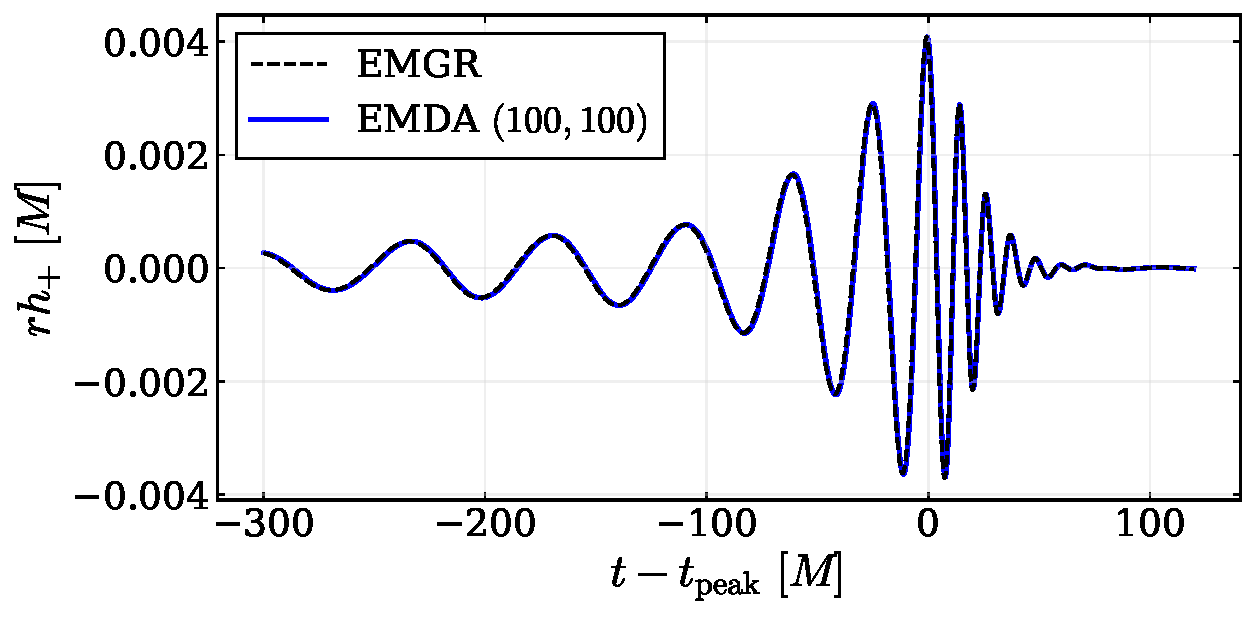
\includegraphics[width=0.85\textwidth]{Figures/Chapter3/em_a0_0_a1_0_vs_emda_a0_100_a1_100_peak_aligned_hplus_notitle.pdf}
\caption{Peak-aligned comparison of the dominant gravitational-wave strain between the Einstein--Maxwell reference waveform, $(\alpha_0,\alpha_1)=(0,0)$, and the strongest-coupling EMDA case, $(\alpha_0,\alpha_1)=(100,100)$. The waveforms agree extremely well, the mismatch of this waveform is on the order of $10^{-5}$}
\label{fig:em_vs_emda_hplus}
\end{figure}
 
\paragraph{Electromagnetic radiation}

We also compare the electromagnetic radiative modes and $\Phi_2$, as introduced in earlier chapters. Rather than computing a mismatch for these modes, we perform a direct comparison of the electromagnetic waveforms. The results show that the waveform differences increase as the coupling strengths are increased. The electromagnetic signal retains the same basic structure across the coupling choices, but its amplitude changes. We display the $++$ charge configuration here, although the other charge configurations show broadly similar behavior.

\begin{figure}[t]
\centering
\subfloat[Real part of $\Phi_2^{22}$.]{
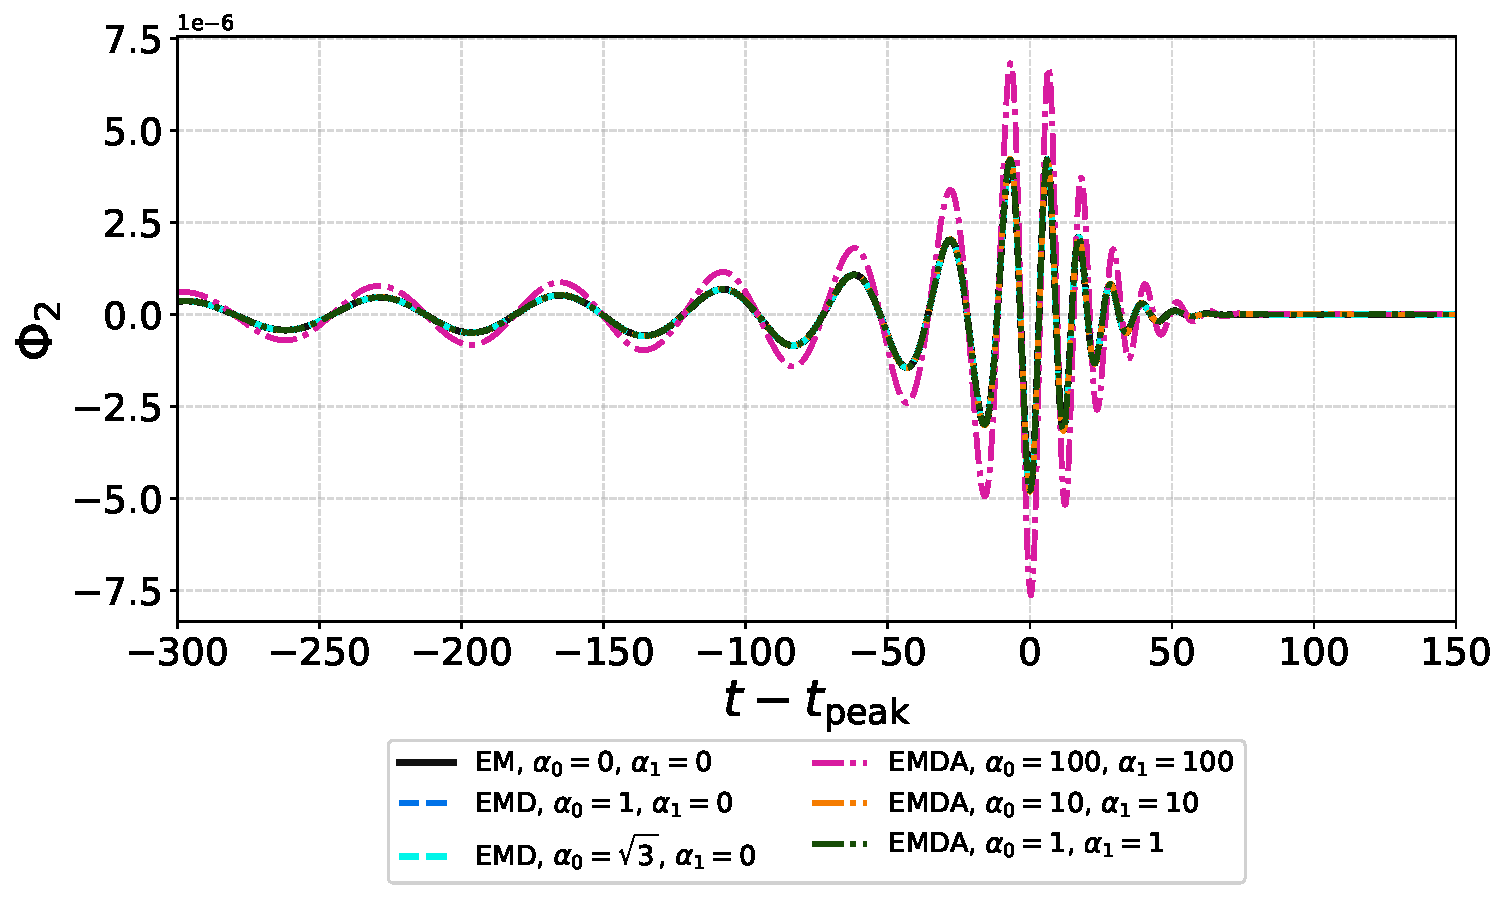
\includegraphics[width=0.48\textwidth]{Figures/Chapter3/PHI2_l2_m2_r5_real.pdf}
}
\hfill
\subfloat[Absolute difference relative to the Einstein--Maxwell case.]{
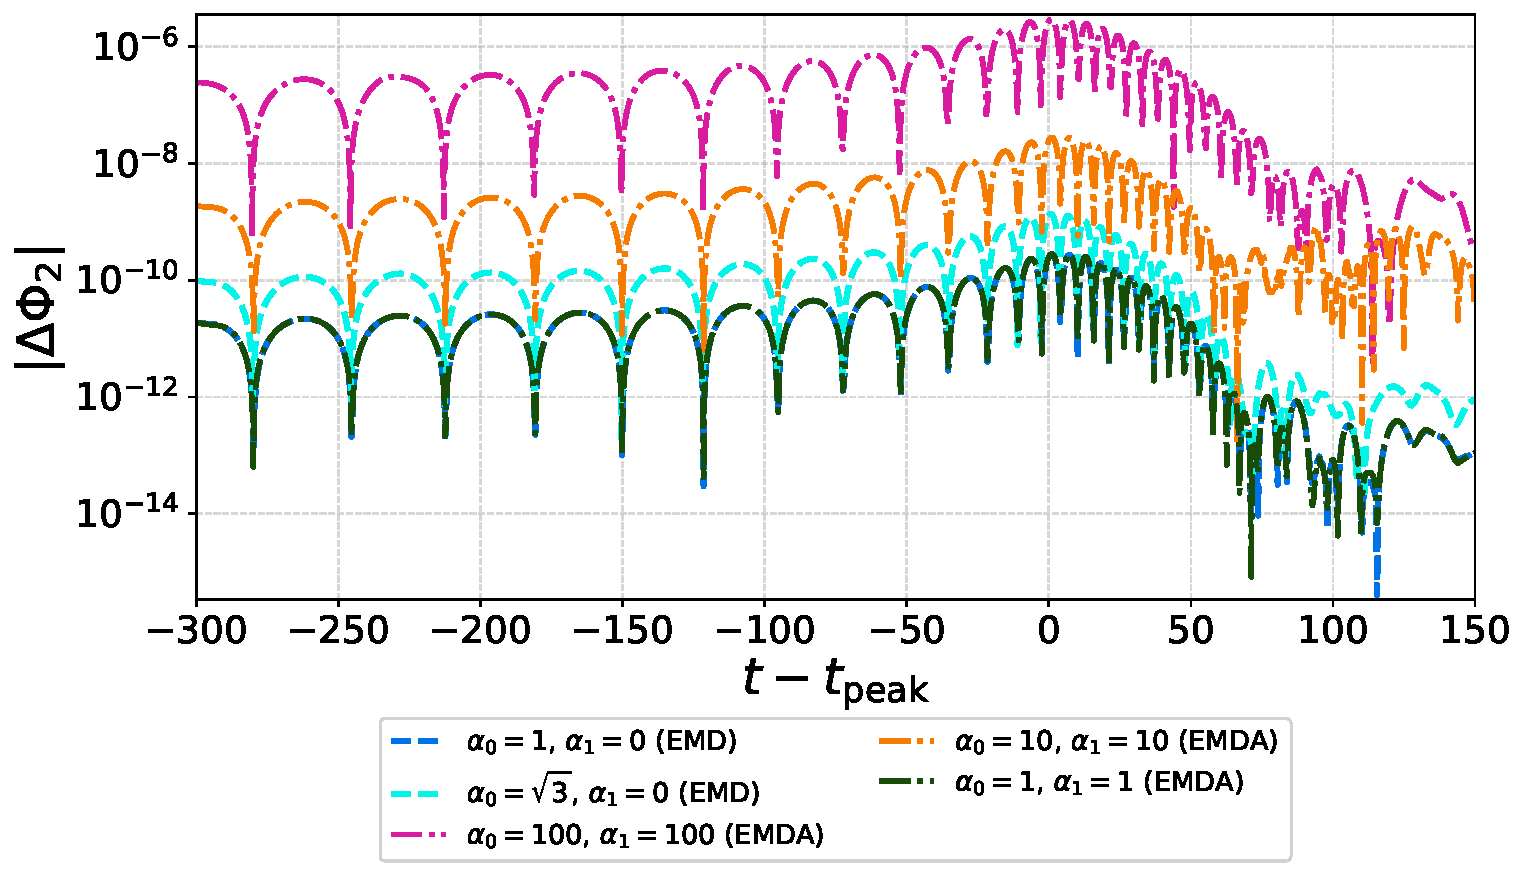
\includegraphics[width=0.48\textwidth]{Figures/Chapter3/PHI2_l2_m2_r5_real_absdiff_vs_EM_log.pdf}
}
\caption{Comparison of the $(\ell,m)=(2,2)$ mode of the electromagnetic scalar $\Phi_2$, extracted at $R_{\mathrm{ex}}=100M$. The left panel shows the peak aligned real part of $\Phi_2^{22}$ across the coupling choices considered, while the right panel shows the absolute difference relative to the Einstein--Maxwell reference case, $(\alpha_0,\alpha_1)=(0,0)$, on a logarithmic scale. The differences in the waveform get larger as the coupling is increased, although it is primarily the amplitude that changes.}
\label{fig:phi2_l2m2_ch3}
\end{figure}


\paragraph{Dilaton radiation}

\begin{figure}[t]
\centering
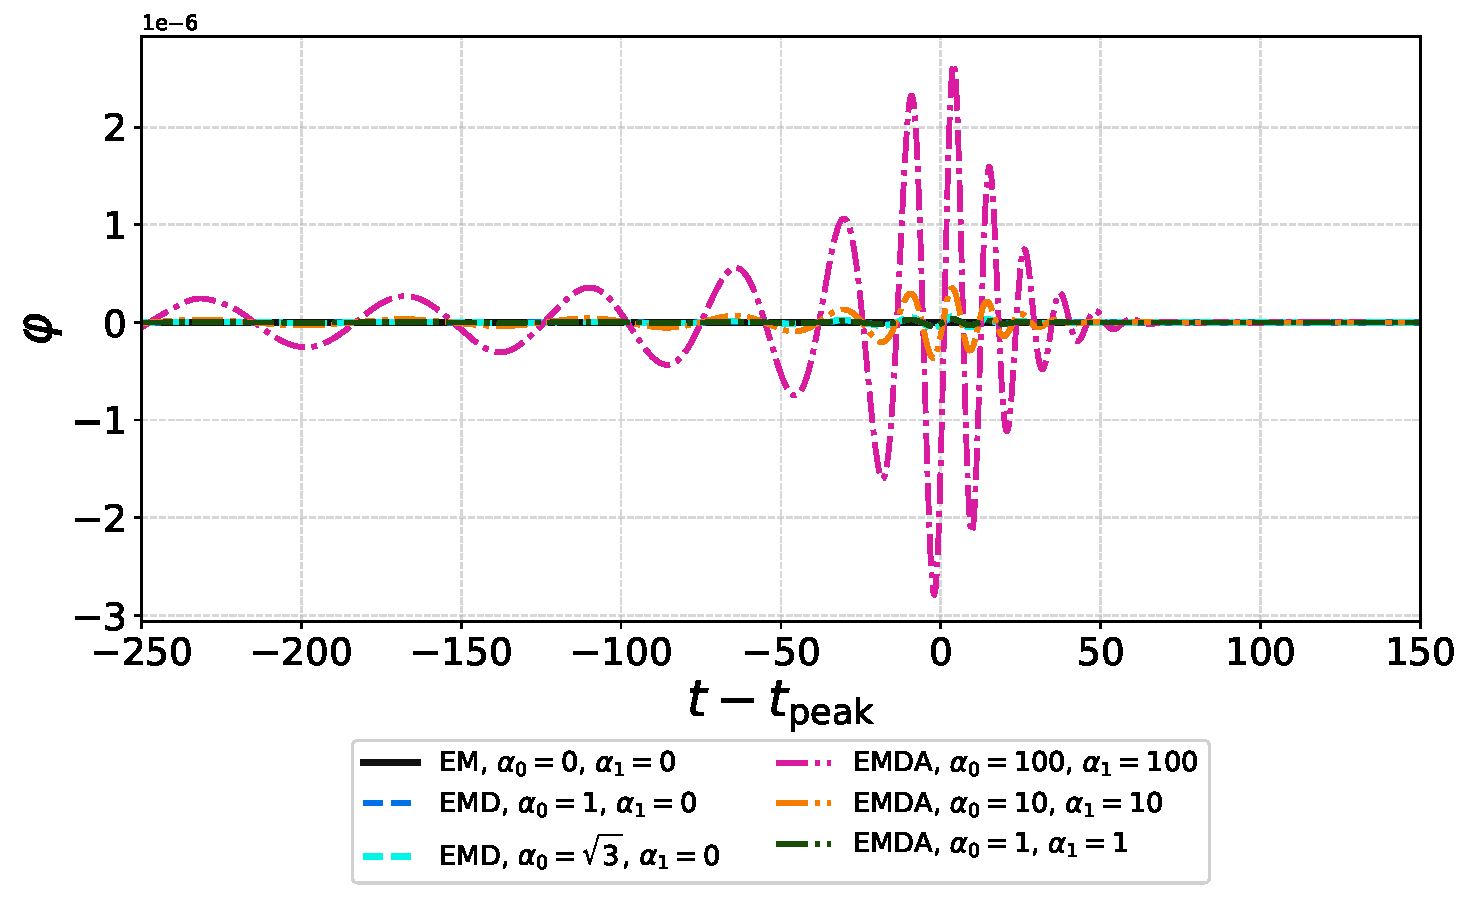
\includegraphics[width=0.48\textwidth]
{Figures/Chapter3/Dilaton_l2_m2_r5_real.pdf}
\caption{
Peak-aligned comparison of the real part of the
$(\ell,m)=(2,2)$ mode of the dilaton radiation,
extracted at $R_{\mathrm{ex}}=100M$, for the coupling
choices considered.
}
\label{fig:dilaton_l2m2_ch3}
\end{figure}

As the coupling strength increases, the amplitude of the emitted
dilaton radiation also increases.


\subsection{Constraints}

Because the initial data are approximate, the constraint violations provide an important check on the quality of the evolutions. We monitor the Hamiltonian constraint, together with the electric and magnetic divergence constraints, throughout the simulations. These quantities are shown in Figs.~\ref{fig:chapter3_hamiltonian_constraint}--\ref{fig:chapter3_divb_constraint}. Across the set of coupling choices considered here, the constraints remain controlled during the initial relaxation, inspiral, and merger. The largest features occur during the early relaxation phase and near merger, where the fields vary most rapidly.

\begin{figure}[t]
\centering
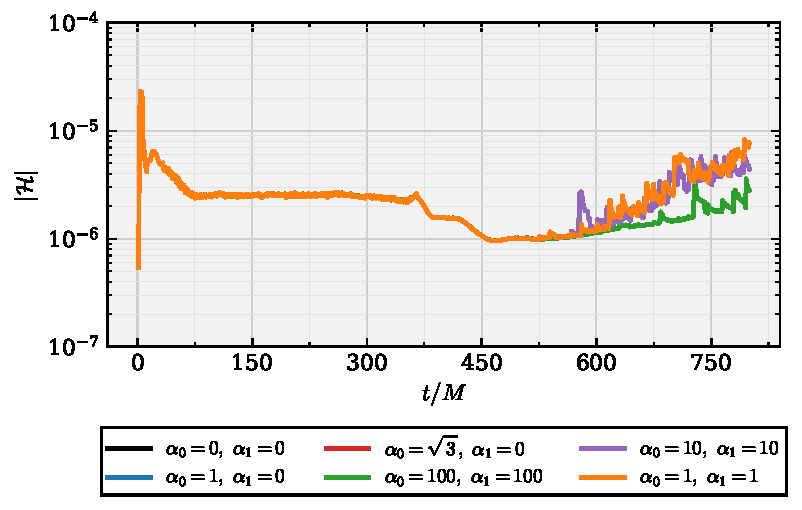
\includegraphics[width=0.85\textwidth]{Figures/Chapter3/all_runs_C_HAM.pdf}
\caption{Hamiltonian constraint violation for the different coupling choices. The curves show the evolution of the Hamiltonian constraint norm for the Einstein--Maxwell reference case and the corresponding EMD and EMDA evolutions. There is an initial spike as the simulations begin, but the constraint quickly settles to a lower value. The Hamiltonian constraint does not show runaway growth and remains low throughout the evolution.}
\label{fig:chapter3_hamiltonian_constraint}
\end{figure}

\begin{figure}[t]
\centering
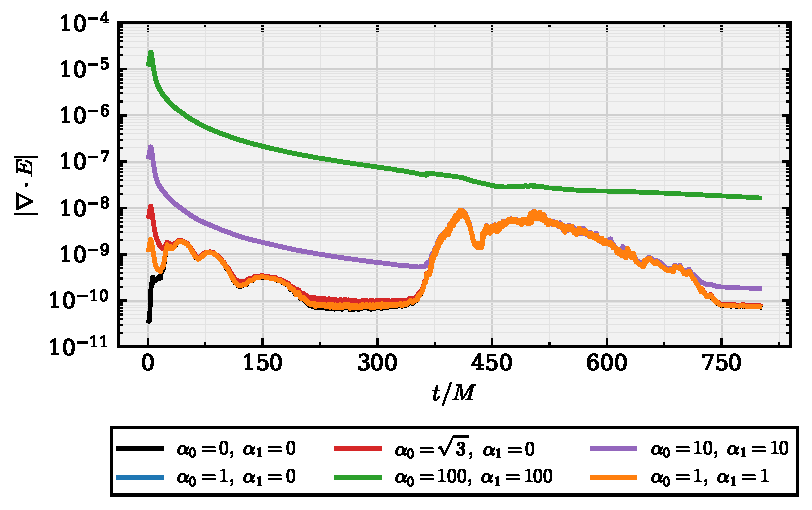
\includegraphics[width=0.85\textwidth]{Figures/Chapter3/all_runs_C_DIVE.pdf}
\caption{Electric divergence constraint violation for the different coupling choices. The curves show the evolution of the electric constraint norm across the Einstein--Maxwell, EMD, and EMDA evolutions. The constraint is initially largest for the strongest coupling, but hyperbolic cleaning reduces it over time. Overall, these constraints remain well behaved throughout the evolution.}
\label{fig:chapter3_dive_constraint}
\end{figure}

\begin{figure}[t]
\centering
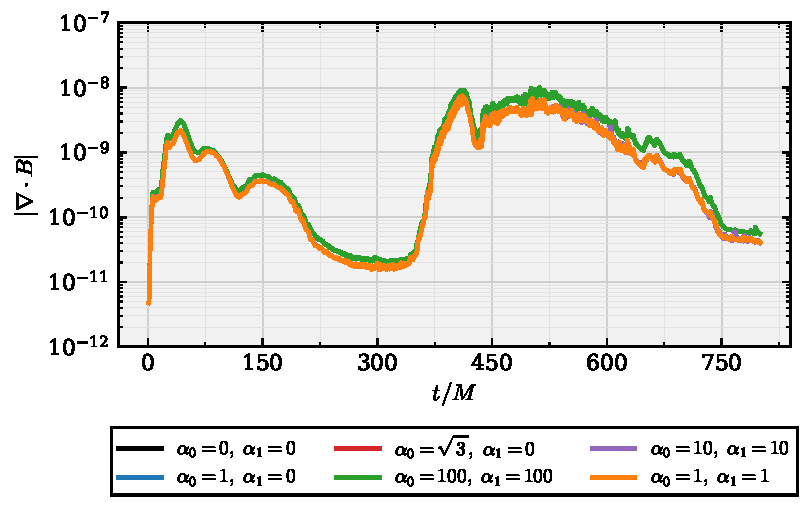
\includegraphics[width=0.85\textwidth]{Figures/Chapter3/all_runs_C_DIVB.pdf}
\caption{Magnetic divergence constraint violation for the different coupling choices. The curves show the evolution of the magnetic constraint norm across the Einstein--Maxwell, EMD, and EMDA evolutions. These values remain low throughout the simulation, providing confidence that the magnetic divergence constraint remains well behaved.}
\label{fig:chapter3_divb_constraint}
\end{figure}

The electromagnetic constraints remain bounded throughout the evolutions, indicating that the divergence-cleaning scheme prevents the electric and magnetic constraint violations from growing without bound. The Hamiltonian constraint shows the expected transient behavior during the initial relaxation and near merger, but it does not exhibit runaway growth. These results indicate that the simulations remain sufficiently well controlled for the qualitative waveform comparisons presented above.

\section{Conclusion}

In this chapter, we studied binary black hole mergers in a broader region of Einstein--Maxwell--dilaton--axion theory by varying the coupling parameters that control the interactions between the electromagnetic, dilaton, and axion fields. We focused primarily on the diagonal sector, $\alpha_0=\alpha_1$, and compared several representative coupling choices against the Einstein--Maxwell reference case. Because exact binary black hole initial data are not available for these theories, we used approximate charged binary black hole initial data and allowed the systems to relax dynamically before merger.

The evolutions remained stable for the coupling choices considered here, and the electromagnetic and gravitational constraints remained controlled throughout the simulations. This provides evidence that the numerical framework can be used to explore binary black hole dynamics beyond the analytically known special cases of EMDA theory. In particular, these simulations provide a first step toward studying how nonlinear merger dynamics depend on the theory's coupling parameters.

For the small charge considered in this study, we found that the dominant gravitational wave signal is only weakly affected by the choice of coupling. The smaller coupling EMD and EMDA cases remained effectively indistinguishable from the Einstein--Maxwell reference waveform at the accuracy of the present simulations. The strongest coupling case, $(\alpha_0,\alpha_1)=(100,100)$, produced the largest departure from the reference waveform, but even this difference remained small in the dominant strain.

The electromagnetic radiation shows a clearer dependence on the coupling parameters. Rather than computing electromagnetic mismatches, we directly compared the radiative modes $\Phi_2$ against the Einstein--Maxwell reference case. These comparisons show that the electromagnetic waveform differences generally increase as the coupling strengths are increased. The overall structure of the electromagnetic signal remains similar across the coupling choices, but the amplitude changes. This behavior is shown for the $++$ charge configuration, with the other charge configurations exhibiting broadly similar patterns.

Taken together, these results suggest that coupling dependent effects are subtle in the gravitational radiation at small charge, but are more visible in the electromagnetic sector. Because the simulations use approximate initial data, very small waveform differences may be affected by relaxation effects, finite resolution error, and waveform extraction uncertainty rather than only by physical coupling dependence. Larger charges, longer inspirals, improved initial data, and explicit convergence tests may be required to clearly separate physical effects from numerical and initial data uncertainties.

Future work could potentially look at improving the initial data by adding axion contributions and improving the initial electric field used in the TPID solver. We could also perform higher charge or higher spin runs to test a wider range of Kerr--Sen configurations. Another study could examine different parts of the EMDA parameter space, including cases where the two couplings are not equal, $\alpha_0 \neq \alpha_1$.

\subsection{Mismatch summary}

\begin{table}[t]
\centering
\begin{tabular}{lccc}
\hline
Theory & $q=0.05,\,+0$ & $q=0.05,\,+-$ & $q=0.05,\,++$ \\
\hline
EMD $(\alpha_0,\alpha_1)=(1,0)$
& $3.85\times 10^{-8}$
& $2.70\times 10^{-7}$
& $4.43\times 10^{-14}$ \\
EMD $(\alpha_0,\alpha_1)=(\sqrt{3},0)$
& $3.53\times 10^{-12}$
& $9.00\times 10^{-8}$
& $2.89\times 10^{-12}$ \\
EMDA $(\alpha_0,\alpha_1)=(1,1)$
& $2.59\times 10^{-8}$
& $6.08\times 10^{-8}$
& $4.92\times 10^{-14}$ \\
EMDA $(\alpha_0,\alpha_1)=(10,10)$
& $7.06\times 10^{-8}$
& $1.22\times 10^{-6}$
& $6.14\times 10^{-10}$ \\
EMDA $(\alpha_0,\alpha_1)=(100,100)$
& $9.62\times 10^{-6}$
& $4.42\times 10^{-5}$
& $3.91\times 10^{-6}$ \\
\hline
\end{tabular}
\caption{Mismatch between the Einstein--Maxwell reference waveform, $(\alpha_0,\alpha_1)=(0,0)$, and the waveforms obtained for different coupling choices. The comparisons use the dominant $\ell=m=2$ gravitational strain mode. The mismatches are small, so most of these waveforms should be considered effectively indistinguishable within the accuracy of the present simulations. In this regime, finite resolution, approximate initial data, and other numerical effects may contribute more to the measured mismatch than the scalar and pseudoscalar fields themselves.}
\label{tab:emda_coupling_mismatches}
\end{table}